\DocumentMetadata{
    tagging=on,
    tagging-setup={math/setup=mathml-SE},
    pdfstandard=ua-2,
    lang=en-US,
}
\documentclass[11pt,english]{article}



\listfiles
\usepackage{fullpage}
\usepackage[showframe=false,margin=1in]{geometry}
\parindent=0pt

\usepackage{relsize}
\usepackage[T1]{fontenc} % for properly hyphenating words with accented chars
\usepackage{babel}

\usepackage{epsfig}
\usepackage{graphicx}
\usepackage{wrapfig}
\usepackage[belowskip=0pt,aboveskip=0pt,font=small]{caption}
\usepackage{subcaption}
\setlength{\intextsep}{7pt plus 0pt minus 0pt}

\usepackage{amsmath, amsthm, amssymb}
\usepackage{textcomp}
\usepackage{stmaryrd}
\usepackage{upgreek}
\usepackage{bm}
\usepackage{cases}
\usepackage{mathtools}

\usepackage{url}
\usepackage{breakurl}
\usepackage[colorlinks=true]{hyperref}
\usepackage{xspace}
\usepackage{comment}
\usepackage{color}
\usepackage{afterpage}
\usepackage[normalem]{ulem}
\usepackage{enumitem}



\usepackage{../assets/mysymbols}
\usepackage{amsmath,amsfonts}
\usepackage{amsthm,amssymb,amsopn}
\usepackage{bm} % bold symbol
\usepackage{bbm}

\newcommand{\vct}[1]{\boldsymbol{#1}} % vector
\newcommand{\mat}[1]{\boldsymbol{#1}} % matrix

\newcommand{\field}[1]{\mathbb{#1}}
\newcommand{\R}{\field{R}} % real domain
\newcommand{\C}{\field{C}} % complex domain
\newcommand{\F}{\field{F}} % functional domain
\newcommand{\T}{^{\textrm T}} % transpose
\newcommand{\TN}{^{-\textrm T}} % transpose
\newcommand{\Lagr}{\mathcal{L}}


\newcommand{\cst}[1]{\mathsf{#1}}

\newcommand{\inner}[2]{#1\cdot #2}
\newcommand{\twonorm}[1]{\|#1\|_2^2}
\newcommand{\Map}[1]{\mathcal{#1}}

\newcommand{\ProbOpr}[1]{\mathbb{#1}}
\newcommand\independent{\protect\mathpalette{\protect\independenT}{\perp}}
\def\independenT#1#2{\mathrel{\rlap{$#1#2$}\mkern2mu{#1#2}}}
\newcommand{\cind}[3]{{#1} \independent{#2}\,|\,#3}
\newcommand{\cndexp}[2]{\ProbOpr{E}\,[ #1\,|\,#2\,]}



\newtheorem{thm}{Theorem}

\newcommand{\eat}[1]{}

\newcommand{\hide}[1]{}

\newcommand{\diff}{\mathop{}\!\mathrm{d}}
\newcommand{\Vop}{\textrm{T}}
\newcommand{\norminf}[1]{\norm{#1}_\infty}

\newcommand{\vecy}{\ensuremath{\mathbf{y}}\xspace}
\newcommand{\vecx}{\ensuremath{\mathbf{x}}\xspace}
\renewcommand{\argmax}{\operatornamewithlimits{argmax}}
\newcommand{\startsym}{\mbox{\scriptsize \texttt{<s>}}\xspace}
\newcommand{\stopsym}{\mbox{\scriptsize \texttt{</s>}}\xspace}
\newcommand{\best}{\ensuremath{\mathit{best}}\xspace}
\newcommand{\bestuptoi}{\ensuremath{\texttt{best}_{\leq i}}\xspace}
\newcommand{\bestuptot}{\ensuremath{\texttt{best}_{\leq t}}\xspace}
\newcommand{\completed}{\ensuremath{\texttt{comp}}\xspace}
\newcommand{\toptop}{\operatornamewithlimits{\mathbf{top}}}
\newcommand{\tuple}[1]{\ensuremath{\langle {#1} \rangle}}
\newcommand{\xuptot}{\ensuremath{\mathit{x}_{\leq t}}\xspace}


\renewcommand{\hide}[1]{}

\begin{document}
\title{CS 4644/7643: Deep Learning\\
Fall 2026 \\
Problem Set 2} 

\author{Instructor: Danfei Xu \\
TAs: Rohan Bansal, Uzu (Chris) Lee, Alfred Cueva  \\
Kun-Lin Hsieh, Chuye Zhang, Liqian Ma, Robert Azarcon  \\
Dhruv Ahuja, Xinchen Yin \\
Discussions: \url{https://piazza.com/class/ms43b2tjxa63lq\#}}
\date{Deadline: Wednesday, October 7 2026, 11:59 pm}
\maketitle


\paragraph*{Instructions}
\begin{enumerate}
\item We will be using Gradescope to collect your assignments. Please read the following instructions for submitting to Gradescope carefully!
     \begin{itemize}
          \item
               For the \textbf{HW2 Theory} component on Gradescope, upload one single PDF containing the answers to all the theory questions. \textbf{However, the solution to each problem/subproblem must be on a separate page. When submitting to Gradescope, please make sure to mark the page(s) corresponding to each problem/sub-problem.}
          \item
               For the \textbf{HW2 Coding - Part 1} on Gradescope, please use the \texttt{collect\_submission.py} script provided and upload \textbf{hw2\_part1\_code\_submission.zip}
          \item
               For the \textbf{HW2 Coding - Part 2} on Gradescope, please use the \texttt{collect\_submission.py} script provided and upload \textbf{hw2\_part2\_code\_submission.zip}
          \item
               For the \textbf{HW2 Notebook} component on Gradescope, please use the \texttt{collect\_submission.py} script provided and upload the resulting \textbf{hw2\_notebook\_submission.pdf} on Gradescope.
          \item
               Note: This is a large class and Gradescope's assignment segmentation features are essential.
               Failure to follow these instructions may result in parts of your assignment not being graded.
               We will not entertain regrading requests for failure to follow instructions.
     \end{itemize}

\item
     \LaTeX'd solutions are strongly encouraged, but scanned handwritten copies are acceptable. Hard copies are \textbf{not} accepted.


\item We generally encourage you to collaborate with other students.

You may talk to a friend,
discuss the questions and potential directions for solving them. However, you need to write
your own solutions and code separately, and \emph{not} as a group activity.
Please list the students you collaborated with. \\ \\

\end{enumerate}
\newpage


\section{Collaborators [0.5 points]}

Please list your collaborators and assign this list to the corresponding section of the outline on Gradescope. If you don't have any collaborators, please write 'None' and assign it to the corresponding section of the Gradescope submission regardless. Not assigning this question on Gradescope or leaving it blank will be marked as zero.

\section{Gradient Descent}
\begin{enumerate}[start=1]

\item
\textbf{[3 points]}

We often use iterative optimization algorithms such as Gradient Descent to
find $\mathbf{w}$ that minimizes a loss function $f(\mathbf{w})$. Recall that in gradient descent,
we start with an initial value of $\mathbf{w}$ (say $\mathbf{w}^{(1)}$) and iteratively take a step in the direction
of the negative of the gradient of the objective function \ie
\begin{equation}
\mathbf{w}^{(t+1)} = \mathbf{w}^{(t)} - \eta\nabla f(\mathbf{w}^{(t)})
\end{equation}
for learning rate $\eta > 0$.

In this question, we will develop a slightly deeper understanding of this update rule, in particular for 
minimizing a convex function $f(\mathbf{w})$. Note: this analysis will not directly carry over to training neural networks 
since loss functions for training neural networks are typically not convex, but this will (a) develop intuition 
and (b) provide a starting point for research in non-convex optimization (which is beyond the scope of this class). 


Recall the first-order Taylor approximation of $f$ at $\mathbf{w}^{(t)}$:
\begin{align}\label{first-order-approx}
f(\mathbf{w}) \approx f(\mathbf{w}^{(t)}) + \langle \mathbf{w}-\mathbf{w}^{(t)},
\nabla f(\mathbf{w}^{(t)}) \rangle
\end{align}
When $f$ is convex, this approximation forms a lower bound of $f$, \ie 
\begin{align}
f(\mathbf{w}) \ge 
\underbrace{
f(\mathbf{w}^{(t)}) + \langle \mathbf{w}-\mathbf{w}^{(t)}, 
\nabla f(\mathbf{w}^{(t)}) \rangle
}_{\text{affine lower bound to $f(\cdot)$}}
 \quad \forall \mathbf{w}
\end{align}

Since this approximation
is a `simpler' function than $f(\cdot)$, we could consider minimizing the approximation instead of $f(\cdot)$.
Two immediate problems: (1) the approximation is affine (thus unbounded from below) and
(2) the approximation is faithful for $\mathbf{w}$ close to $\mathbf{w}^{(t)}$.
To solve both problems, we add a squared $\ell_2$ \emph{proximity term} to the approximation minimization:
\begin{equation}
\argmin_\mathbf{w}
\underbrace{
f(\mathbf{w}^{(t)}) + \langle \mathbf{w}-\mathbf{w}^{(t)}, \nabla f(\mathbf{w}^{(t)}) \rangle
}_{\text{affine lower bound to $f(\cdot)$}}
+
\underbrace{
\frac{\lambda}{2}
}_{\text{trade-off}}
\underbrace{
\norm{\mathbf{w} - \mathbf{w}^{(t)}}^2
}_{\text{proximity term}}
\end{equation}

Notice that the optimization problem above is an unconstrained quadratic programming problem,
meaning that it can be solved in closed form (hint: gradients).

What is the solution $\mathbf{w}^*$ of the above optimization?
What does that tell you about the gradient descent update rule?
What is the relationship between $\lambda$ and $\eta$?


\end{enumerate}

\newpage
\section{Convolutions}
\begin{enumerate}[resume]

\item 
\textbf{[4 points]}

\textbf{Transposed Convolution} is an upsampling operation used in tasks such as image segmentation and generative models. Unlike standard convolution which downsamples the input, transposed convolution expands the spatial dimensions. The following figure shows transposed convolution with input $ x \in \mathbb{R}^{2 \times 2}$, kernel $ w \in \mathbb{R}^{3 \times 3}$, and output $ y \in \mathbb{R}^{4 \times 4}$. You may find this \href{https://d2l.ai/chapter_computer-vision/transposed-conv.html}{link} helpful for understanding the operation in-depth.

\begin{figure}[h!]
    \centering
    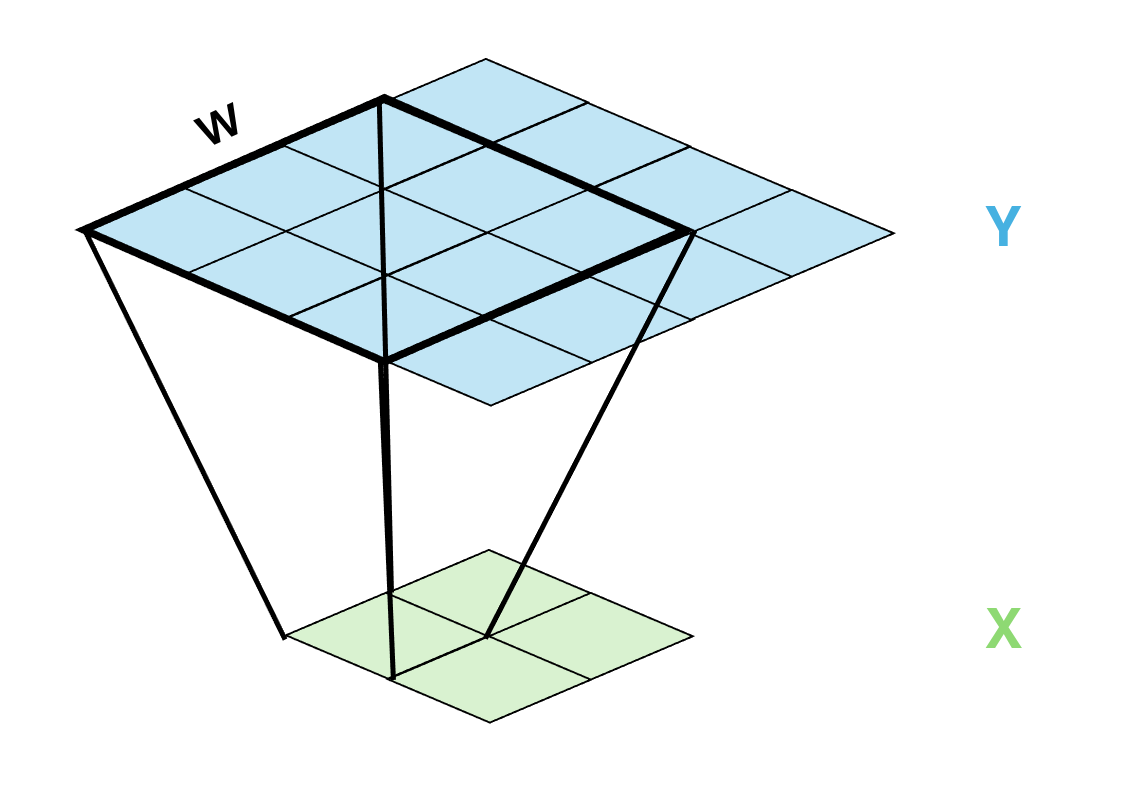
\includegraphics[scale=0.2]{assets/transposed_conv.png}
\end{figure}

\textbf{Problem:}
Assume input $ x \in \mathbb{R}^{3 \times 3}$ and kernel $ w \in \mathbb{R}^{3 \times 3}$. When transposed convolution with stride 2 is applied, the resulting output $\textbf{y}$ will have dimensions $7 \times 7$.
The gradient of the loss $L$ with respect to the output $y$ is given as $\delta = \frac{\partial L}{\partial y} \in \mathbb{R}^{7 \times 7}$.

\vspace{0.5cm}
(a) \textbf{[1 point]} Compute output y with following given input x and kernel w.

\textbf{Given:}
\[
w = \begin{bmatrix} 
0 & 0 & 0 \\ 
0 & 1 & 2 \\ 
3 & 4 & 5 
\end{bmatrix}, \quad
x = \begin{bmatrix} 
1 & 1 & 1 \\ 
1 & 1 & 1 \\ 
1 & 1 & 1
\end{bmatrix} 
\]
\textbf{Compute:}
\[
y = 
\begin{bmatrix} 
\quad \quad & \quad \quad & \quad \quad \\ \\
\quad \quad & \quad \quad & \quad \quad \\ \\
\quad \quad & \quad \quad & \quad \quad 
\end{bmatrix}
\]








\vspace{1cm}

(b) \textbf{[1 point]} Assume the following simple values for the kernel $w$ and the gradient $\delta$. Calculate $\frac{\partial L}{\partial x}$. (Hint : It can be simplified by convolution or transposed convolution between the two given matrices)

\textbf{Given:}
\[
w = \begin{bmatrix} 
0 & 0 & 0 \\ 
0 & 1 & 2 \\ 
3 & 4 & 5 
\end{bmatrix}, \quad
\delta = \begin{bmatrix} 
0 & 0 & 0 & 2 & 0 & 0 & 0 \\
0 & 3 & 0 & 0 & 0 & 3 & 0 \\
0 & 0 & 0 & 0 & 0 & 0 & 0 \\
2 & 0 & 0 & 0 & 0 & 0 & 2 \\
0 & 0 & 0 & 0 & 0 & 0 & 0 \\
0 & 3 & 0 & 0 & 0 & 3 & 0 \\
0 & 0 & 0 & 2 & 0 & 0 & 0 
\end{bmatrix} 
\]
\textbf{Calculate:}

\[
\frac{\partial L}{\partial x} = 
\begin{bmatrix} 
\quad \quad & \quad \quad & \quad \quad \\ \\
\quad \quad & \quad \quad & \quad \quad \\ \\
\quad \quad & \quad \quad & \quad \quad 
\end{bmatrix}
\]
\vspace{1cm}


(c) \textbf{[1 point]} Assume the following simple values for the input $x$ and the gradient $\delta$. Calculate $\frac{\partial L}{\partial w}$. \textbf{Be careful that $x$ here is different from (a).} (Hint : Similar to (b), it can be simplified by convolution or transposed convolution but it may need some manipulation on given matrix)

\textbf{Given:}
\[
x = \begin{bmatrix} 
1 & 0 & 1 \\ 
0 & 1 & 0 \\ 
1 & 0 & 1 
\end{bmatrix} \quad , 
\delta = \begin{bmatrix} 
0 & 0 & 0 & 2 & 0 & 0 & 0 \\
0 & 3 & 0 & 0 & 0 & 3 & 0 \\
0 & 0 & 0 & 0 & 0 & 0 & 0 \\
2 & 0 & 0 & 0 & 0 & 0 & 2 \\
0 & 0 & 0 & 0 & 0 & 0 & 0 \\
0 & 3 & 0 & 0 & 0 & 3 & 0 \\
0 & 0 & 0 & 2 & 0 & 0 & 0 
\end{bmatrix} 
\]


\textbf{Calculate:}

\[
\frac{\partial L}{\partial w} = 
\begin{bmatrix} 
\quad \quad & \quad \quad & \quad \quad \\ \\
\quad \quad & \quad \quad & \quad \quad \\ \\
\quad \quad & \quad \quad & \quad \quad 
\end{bmatrix}
\]

\vspace{1cm}

(d) \textbf{[1 point] (Required for 7643; Extra Credit for 4644)}

In the original U-Net architecture (Ronneberger et al., 2015), \textbf{Transposed Convolution} (often referred to as up-convolution) was used to upsample feature maps. However, in modern generative models (e.g., GANs), this operation can sometimes introduce grid-like patterns known as "checkerboard artifacts."
\vspace{0.5cm}

\textbf{Question:} 

Consider a 2D Transposed Convolution with Kernel Size $k=8$ and Stride $s=3$.

\textbf{Explain} why some pixels in the output $y$ receive contributions from more input pixels than others. Based on your explanation, \textbf{suggest a stride($\ne$1)} to avoid this uneven overlap (i.e., to avoid checkerboard artifacts).
\end{enumerate}

\newpage
\section{Initialization}
\begin{enumerate}[resume]
\item 
\textbf{[3 points + 2 points]}

Proper weight initialization is critical for training deep networks. If activations grow or shrink as they propagate through layers, training becomes unstable. In this problem, we will derive some common initialization schemes. You may find that completing the paper review for this assignment will help with this problem.

Consider a deep network with layers $h^{(l)} = W^{(l)} h^{(l-1)}$, ignoring biases for now. Here $h^{(l)} \in \mathbb{R}^{n_{\text{out}}}$ is a column vector of activations, and the weight matrix $W^{(l)} \in \mathbb{R}^{n_{\text{out}} \times n_{\text{in}}}$ maps $n_{\text{in}}$ inputs to $n_{\text{out}}$ outputs.

Assume:
\begin{itemize}
    \item Inputs $h^{(0)}$ are i.i.d. with zero mean and variance $\text{Var}(h^{(0)}) = \sigma^2$
    \item Weights are initialized i.i.d. with zero mean and variance $\text{Var}(W^{(l)})$
    \item Inputs and weights are independent
    \item You can directly use standard probability identities for expectations and variance
\end{itemize}

\begin{enumerate}[label=(\alph*)]

\item \textbf{[1 point]}

We first analyze how variance changes through a single linear layer. Show that:
\[
\text{Var}(h^{(1)}) = n_{\text{in}} \cdot \text{Var}(W^{(1)}) \cdot \sigma^2
\]

\item \textbf{[1 point]} 

Using your result from part (a), determine what $\text{Var}(W^{(l)})$ should be to ensure the variance is preserved, i.e., $\text{Var}(h^{(1)}) = \text{Var}(h^{(0)})$. This is known as \textbf{Xavier initialization}.

\item \textbf{[1 point]} 

Modern networks use nonlinear activations. Before deriving the appropriate initialization for ReLU networks, we need a key identity. Let $x$ be a random variable with a symmetric distribution with zero mean. Prove that:
\[
\mathbb{E}[\text{ReLU}(x)^2] = \frac{1}{2}\mathbb{E}[x^2]
\]

\item \textbf{[2 points] (Required for 7643: Extra Credit for 4644)} 

Now consider a network with ReLU activations: $h^{(l)} = W^{(l)} \text{ReLU}(h^{(l-1)})$. Using your result from part (c), derive the initialization variance $\text{Var}(W^{(l)})$ needed to to ensure the variance is preserved, i.e., $\text{Var}(h^{(1)}) = \text{Var}(h^{(0)})$. This is known as \textbf{Kaiming initialization}.
\end{enumerate}

\end{enumerate}

\newpage
\section{Paper Review}
\begin{enumerate}[resume]

\item 
\textbf{[4 points]}

\textbf{`Delving Deep into Rectifiers: Surpassing Human-Level Performance on ImageNet Classification'} by \textbf{Kaiming He, et al}. 

The paper examines the fundamental importance of rectifier neural networks and proper initialization for training very deep networks. The study also presents, using experimental results, the PReLU networks (PReLU-nets), which was the first neural network to surpass human-level performance on ImageNet classification. The paper can be viewed \href{https://arxiv.org/abs/1502.01852}{here}.

The evaluation rubric for this section is as follows:

\begin{enumerate}[resume]
\item
\textbf{[2 points]}
Briefly summarize the key contributions, strengths and weaknesses of this paper.

\item
\textbf{[2 points]}
What is your personal takeaway from this paper? This could be expressed either in terms of relating the approaches adopted in this paper to your traditional understanding of image classification networks, or potential future directions of research in the area which the authors haven't addressed, or anything else that struck you as being noteworthy. 
\end{enumerate}

\textbf{Guidelines}: Please restrict your reviews to no more than 350 words (total length for answers to both the above questions).

\end{enumerate}

\end{document}